%!TEX root = ../../main.tex

\chapter{Crystal Quality of Nanodiamonds}	\label{ch::crystal_quality}
\chaptermark{Crystal Quality}

Crystal quality is the a measure for how close a crystal resembles its pristine form\cite{}.
Vacancies, impurity atoms and contamination with graphite or amorphous carbon are examples for factors which decrease the crystal quality \todo[fancyline]{stimmt das?}.
Poor crystal quality may manifest itselves self in \pl spectra as a broad \bkg.
To improve crystal quality, two methods were used: annealing in vacuum and oxidation in air.
We also investigated the effect of oxidation on the Raman spectrum.
Further Raman measurements of various samples give further insight to crystal quality and surface contamination.
At last, several TEM measurements exhibit the composition of the wet-milled \nds. 

	\section{Annealing and Oxidation}\label{sec::ann_ox}

	At temperatures above \todo[fancyline]{enter value}, vacancies in the diamond lattice become mobile and diffuse towards the surface\cite{}.
	During \si implantation the diamond lattice gets damaged by the penetrating ions.
	To reduce the damage in the diamond lattice, we anneal the implanted diamonds at \SI{900}{\celsius} for \SIrange{3}{6}{h} in vacuum (\SI{e-6}{Pa}).
	\\
	The surface of the \nds is contaminated with graphite and amorphous sp$^2$ hybridized carbon \todo[fancyline]{warum}.
	The vacancies which diffuse towards the surface during annealing further increase the amorphous carbon content on the surface of the \nds \cite{}.
	We apply oxidation in a furnace under ambient air at a temperature of \SI{450}{\celsius} for \SIrange{3}{6}{h}.


	\section{Raman Measurements} \label{sec::raman}


		\begin{figure}
			\begin{subfigure}[tp]{0.45\linewidth}
				\caption{}\label{subfig::raman_no}
				\centering
				\testbox{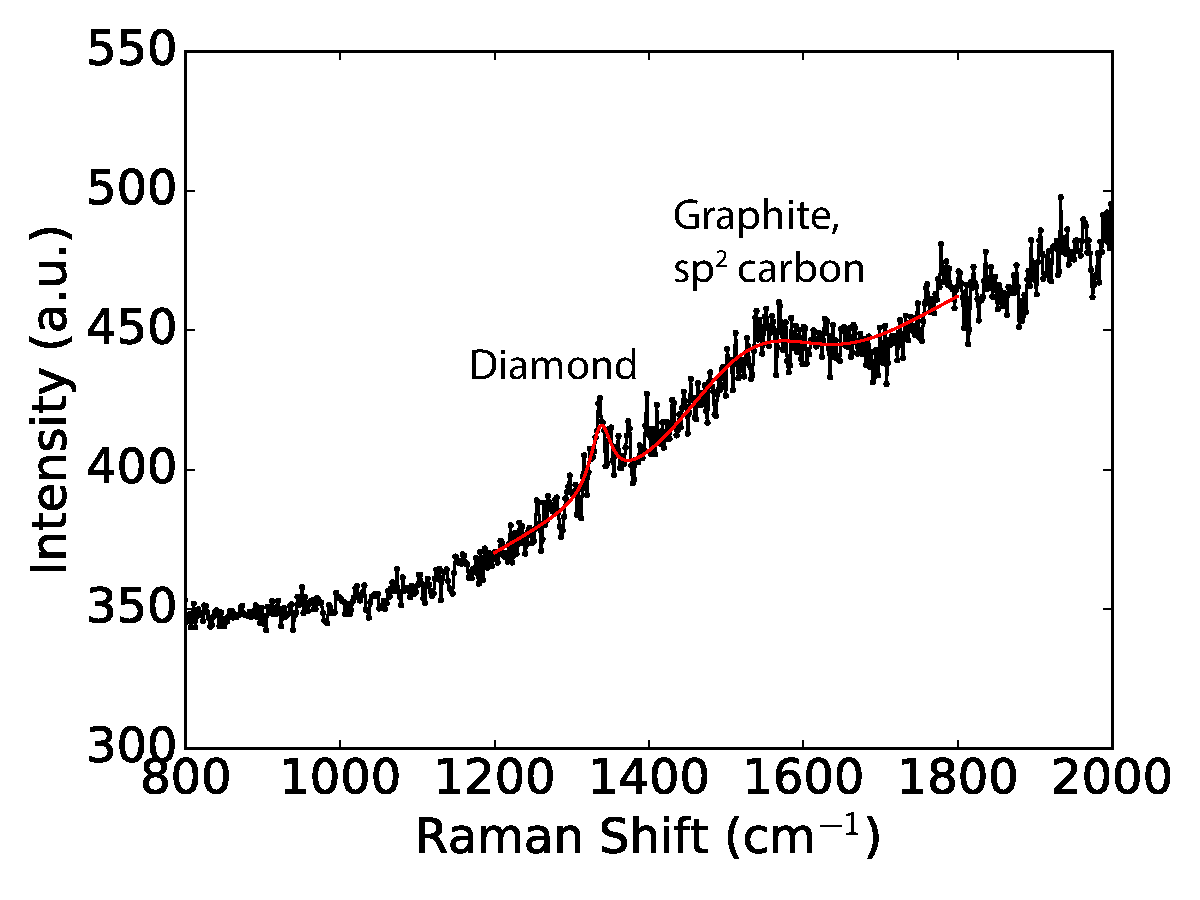
\includegraphics[trim = 0 0 0 0 , clip = true, width = \linewidth]{./pics/Ir25_spectrum_scan_xy-05x6y8_4000uW_t60_wavenumber_fit.pdf}}
			\end{subfigure}
			\hfill
			\begin{subfigure}[tp]{0.45\linewidth}
				\caption{}\label{subfig::raman_ox}
				\centering
				\testbox{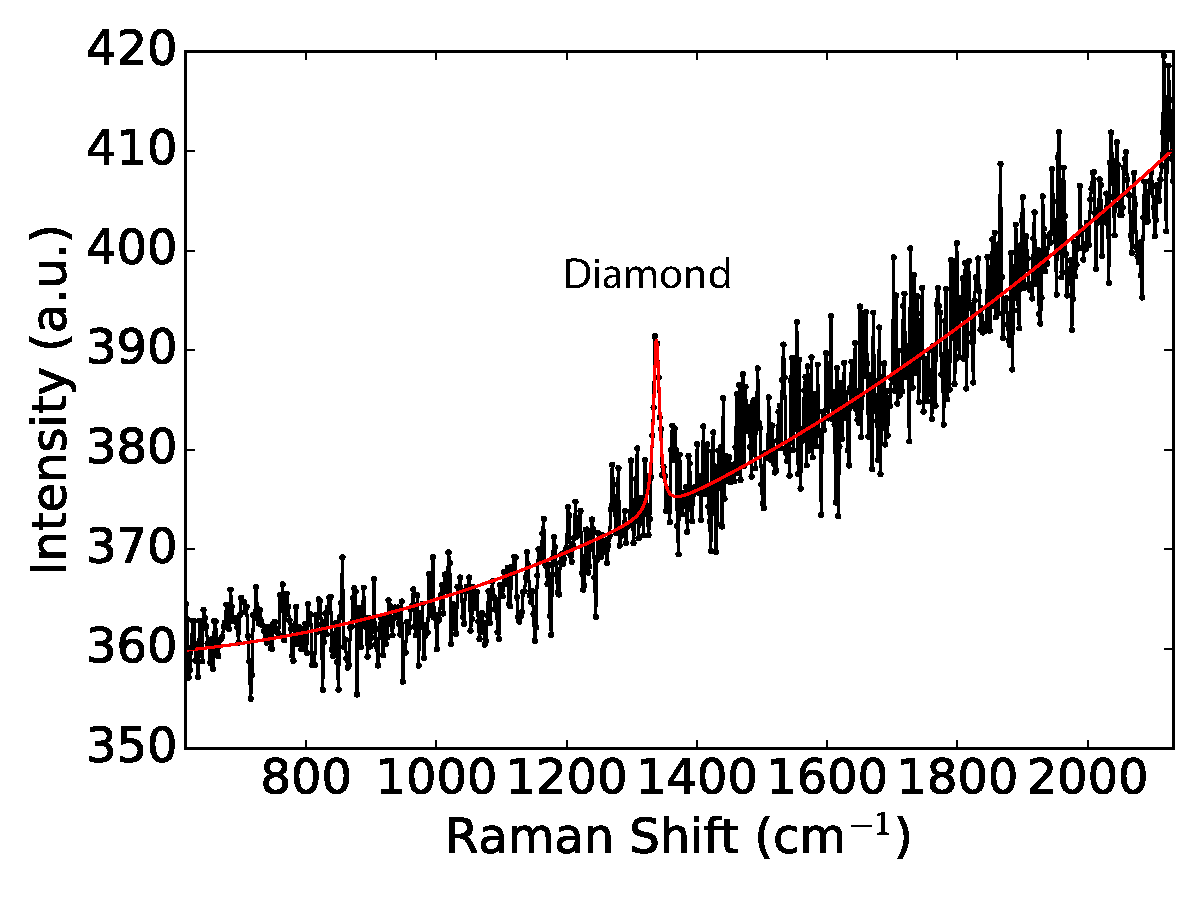
\includegraphics[trim = 0 0 0 0,  clip = true, width = \linewidth]{./pics/Ir_22_spe_scan_xy-02x7y7_550-600nm_t240_wavenumber_fit.pdf}}
			\end{subfigure}
			\caption{Raman measurements, black: data, red: fit. (a) Raman measurement before oxidation, sample \insituS. The diamond Raman peak is situated at \SI{1338}{\per\centi\meter}. The broad feature around \SI{1600}{\per\centi\meter} corresponds to the graphite G-band. (b) Raman measurement after oxidation, sample \insituSo. The G-band has vanished, indicating removal of graphite and amorphous sp$^2$ hybridized carbon.}
			\label{fig::raman}
		\end{figure}

		Raman measurements of the wet-milled \nds give insight to the issues of surface contamination, defects in the diamond lattice and strain in the lattice:
		Surface contamination like graphite and amorphous sp$^2$ hybridized carbon atoms cause additional peaks in the Raman spectrum; a high defect concentration may lead to both additional peaks, to a broadening of the first order Raman peak and a shifts it to smaller wavenumbers; while strain in the diamond broadens the first order Raman peak and causes a shift to higher wavenumbers \cite{Zaitsev2001,Prawer2004,Orwa2000}.
		\\
		As excitation laser a \SI{532}{\nano\meter} continuous wave diode laser is used.
		Due to the low signal from a single \nd, the Raman measurements are carried out at several areas on the sample \insituS which are densely covered with \nds, hence taking measurements of clusters of \nds.
		The narrow peak in \autoref{subfig::raman_no} corresponds to the first order diamond Raman peak.
		The Raman shift of \SI{1338}{\per\centi\meter} compared to the literature value of \SI{1332}{\per\centi\meter} of pristine diamond \cite{Zaitsev2001} indicates the presence of strain in the diamond particles.
		Furthermore, the investigated Raman spectra show a broad peak with a Raman shift of about \SI{1582}{\per\centi\meter} (\autoref{subfig::raman_no}).
		This shift corresponds to the G-band due to amorphous sp$^2$ hybridized carbon atoms and graphite.
		The exact G-band position and \lw is sensitive to parameters such as the clustering of the sp$^2$ phase, bond-length and bond-angle disorder, presence of sp$^2$ rings or chains, and the sp$^2$/sp$^3$ ratio \cite{Ferrari2004}.
		\\
		The \nd Raman spectra are considerably modified after \ox in air at \SI{450}{\degreeCelsius}.
		To verify this, we perform Raman measurements on three different spots on a non-oxidized sample (\insituS), and for comparison on three different spots on a sample produced in the same process which is additionally oxidized.
		While the G-band peak is present in every measurement performed on the sample which was not oxidized, it is not present in any of the measurements performed after \ox (\autoref{subfig::raman_ox}), indicating successful removal of sp$^2$ hybridized carbon and surface graphite.
		The position of the diamond Raman peak is the same oxidized (\insituSo) and non-oxidized (\insituSn) samples, indicating no effect on strain in the diamond.
		On the other hand, the width of the diamond Raman peak is between \SIlist{15; 30}{\per\centi\meter} without \ox treatment, but is only \SIrange{9}{11}{\per\centi\meter} after the \ox process.
		A possible reason for a change of the width is improved crystal quality, as explained in more detail in the following paragraphs.
		\\
		For comparison, measurements of the Raman line were also carried out on the implanted sample \implantedTao. 
		These diamond particles are big enough to perform measurements on single \nds.
		We found diamond one Raman line at \SI[separate-uncertainty]{1308+-5}{\per\centi\meter}, one at \SI[separate-uncertainty]{1345+-5}{\per\centi\meter} and one at \SI[separate-uncertainty]{1348+-5}{\per\centi\meter} (given uncertainties are governed by spectrometer resolution).
		We have to distinguish two cases, a shift of the first order Raman line to higher versus lower wavenumbers than the first order Raman line of \SI{1332}{\per\centi\meter} in pristine diamond.
		\\
		As mentioned above, a Raman shift of the first order Raman line to lower wavenumbers and a broadening of the Raman line indicates defects in the diamond lattice \cite{Prawer2004}.
		The Raman line at \SI[separate-uncertainty]{1308+-5}{\per\centi\meter} exhibits a broad \lw of \SI[separate-uncertainty]{25+-5}{\per\centi\meter}.
		Therefore both the position and the \lw of the Raman line indicate that there are many defects in the diamond.
		\\
		The other case is a shift of the first order Raman line towards higher wavenumbers.
		The shift of the first order Raman line to higher wavenumbers is attributed to strain in the diamond lattice.
		While under hydrostatic pressure, the triply degenerate first order Raman peak remains degenerate, under uniaxial and more complex stress configurations (biaxial stress, shear stress etc.) mode splitting occurs \cite{Prawer2004}.
		As the measured peaks at wavenumbers higher than the wavenumber in pristine diamond are broad, we attribute these peaks to stress configurations other than hydrostatic stress, where the mode splitting manifests itself in a broadening of the peak due to limited spectrometer resolution.
		\\
		To summarize, there are two cases, one where the first order Raman line hints that there are many defects present in the diamond lattice and the other that leads to the assumption that the stress configuration in the diamonds are uniaxial or more complicated stress configurations.
		In \autoref{subsec::spectra} we will show that both of these assumptions fit nicely to the results from the measured \pl spectra. 
